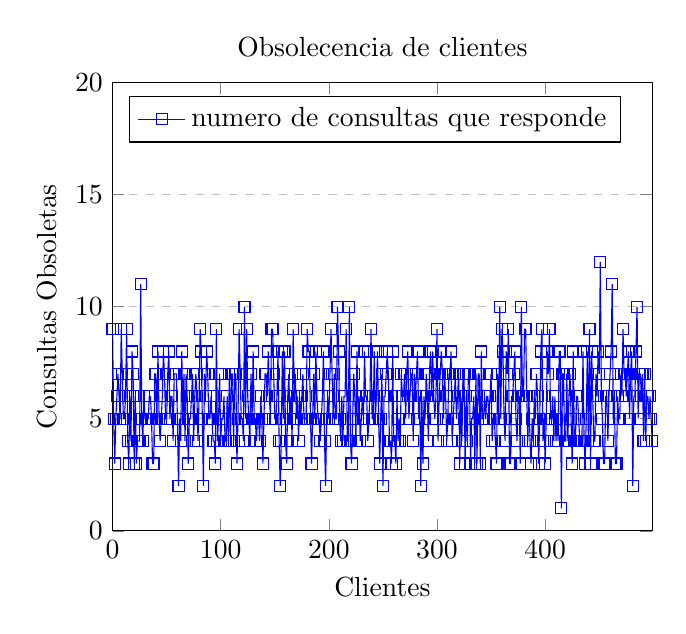
\begin{tikzpicture}
\begin{axis}[
    title={Obsolecencia de clientes},
    xlabel={Clientes},
    ylabel={Consultas Obsoletas},
    xmin=0, xmax=499,
    ymin=0, ymax=20,
    xtick={},
    ytick={},
    legend pos=north west,
    ymajorgrids=true,
    grid style=dashed,
]

\addplot[
    color=blue,
    mark=square,
    ]
    coordinates {
   (0,9)
(1,5)
(2,3)
(3,5)
(4,6)
(5,7)
(6,6)
(7,5)
(8,9)
(9,7)
(10,5)
(11,5)
(12,6)
(13,9)
(14,4)
(15,3)
(16,6)
(17,4)
(18,8)
(19,7)
(20,3)
(21,6)
(22,3)
(23,4)
(24,4)
(25,4)
(26,11)
(27,5)
(28,4)
(29,6)
(30,5)
(31,5)
(32,5)
(33,5)
(34,6)
(35,6)
(36,5)
(37,3)
(38,3)
(39,7)
(40,7)
(41,5)
(42,8)
(43,5)
(44,4)
(45,5)
(46,6)
(47,8)
(48,7)
(49,5)
(50,5)
(51,7)
(52,8)
(53,5)
(54,6)
(55,6)
(56,4)
(57,7)
(58,7)
(59,7)
(60,5)
(61,2)
(62,5)
(63,4)
(64,8)
(65,5)
(66,7)
(67,4)
(68,7)
(69,6)
(70,3)
(71,5)
(72,5)
(73,6)
(74,7)
(75,4)
(76,6)
(77,7)
(78,6)
(79,4)
(80,6)
(81,9)
(82,8)
(83,5)
(84,2)
(85,7)
(86,6)
(87,8)
(88,7)
(89,5)
(90,5)
(91,6)
(92,5)
(93,4)
(94,4)
(95,3)
(96,9)
(97,4)
(98,5)
(99,7)
(100,4)
(101,5)
(102,5)
(103,6)
(104,4)
(105,4)
(106,6)
(107,4)
(108,7)
(109,4)
(110,7)
(111,7)
(112,4)
(113,7)
(114,7)
(115,3)
(116,5)
(117,9)
(118,7)
(119,5)
(120,5)
(121,4)
(122,10)
(123,5)
(124,9)
(125,6)
(126,5)
(127,4)
(128,7)
(129,5)
(130,8)
(131,5)
(132,5)
(133,4)
(134,5)
(135,5)
(136,4)
(137,6)
(138,5)
(139,3)
(140,5)
(141,7)
(142,7)
(143,6)
(144,8)
(145,6)
(146,5)
(147,9)
(148,9)
(149,7)
(150,5)
(151,5)
(152,6)
(153,8)
(154,4)
(155,2)
(156,4)
(157,8)
(158,5)
(159,8)
(160,4)
(161,3)
(162,6)
(163,7)
(164,5)
(165,6)
(166,4)
(167,9)
(168,6)
(169,7)
(170,5)
(171,6)
(172,4)
(173,6)
(174,5)
(175,6)
(176,7)
(177,5)
(178,5)
(179,5)
(180,9)
(181,8)
(182,8)
(183,5)
(184,3)
(185,5)
(186,7)
(187,5)
(188,8)
(189,6)
(190,5)
(191,5)
(192,4)
(193,5)
(194,6)
(195,8)
(196,4)
(197,2)
(198,5)
(199,6)
(200,5)
(201,7)
(202,9)
(203,7)
(204,5)
(205,7)
(206,5)
(207,5)
(208,10)
(209,8)
(210,5)
(211,4)
(212,6)
(213,4)
(214,6)
(215,6)
(216,9)
(217,4)
(218,4)
(219,10)
(220,4)
(221,3)
(222,5)
(223,7)
(224,6)
(225,4)
(226,8)
(227,5)
(228,6)
(229,4)
(230,5)
(231,6)
(232,5)
(233,8)
(234,6)
(235,6)
(236,4)
(237,5)
(238,6)
(239,9)
(240,5)
(241,5)
(242,8)
(243,5)
(244,6)
(245,8)
(246,5)
(247,3)
(248,5)
(249,7)
(250,2)
(251,6)
(252,6)
(253,7)
(254,8)
(255,7)
(256,4)
(257,4)
(258,3)
(259,8)
(260,4)
(261,4)
(262,3)
(263,6)
(264,4)
(265,5)
(266,4)
(267,7)
(268,6)
(269,6)
(270,7)
(271,5)
(272,7)
(273,8)
(274,5)
(275,6)
(276,7)
(277,7)
(278,4)
(279,7)
(280,6)
(281,7)
(282,8)
(283,5)
(284,6)
(285,2)
(286,6)
(287,3)
(288,6)
(289,5)
(290,7)
(291,6)
(292,4)
(293,7)
(294,8)
(295,6)
(296,8)
(297,6)
(298,5)
(299,6)
(300,9)
(301,4)
(302,6)
(303,7)
(304,8)
(305,7)
(306,5)
(307,7)
(308,6)
(309,4)
(310,5)
(311,7)
(312,7)
(313,8)
(314,4)
(315,5)
(316,6)
(317,7)
(318,5)
(319,6)
(320,7)
(321,3)
(322,6)
(323,4)
(324,7)
(325,7)
(326,3)
(327,6)
(328,4)
(329,7)
(330,7)
(331,3)
(332,5)
(333,5)
(334,6)
(335,3)
(336,7)
(337,3)
(338,7)
(339,7)
(340,3)
(341,8)
(342,5)
(343,5)
(344,6)
(345,5)
(346,6)
(347,6)
(348,5)
(349,6)
(350,7)
(351,4)
(352,5)
(353,5)
(354,4)
(355,3)
(356,7)
(357,5)
(358,10)
(359,5)
(360,9)
(361,8)
(362,5)
(363,4)
(364,8)
(365,7)
(366,9)
(367,3)
(368,3)
(369,6)
(370,6)
(371,7)
(372,8)
(373,5)
(374,4)
(375,6)
(376,6)
(377,3)
(378,10)
(379,6)
(380,6)
(381,9)
(382,9)
(383,6)
(384,4)
(385,6)
(386,4)
(387,3)
(388,5)
(389,4)
(390,6)
(391,5)
(392,7)
(393,6)
(394,3)
(395,5)
(396,8)
(397,9)
(398,4)
(399,5)
(400,3)
(401,5)
(402,8)
(403,7)
(404,9)
(405,5)
(406,5)
(407,6)
(408,4)
(409,6)
(410,4)
(411,5)
(412,4)
(413,8)
(414,8)
(415,1)
(416,7)
(417,7)
(418,4)
(419,4)
(420,7)
(421,4)
(422,6)
(423,7)
(424,5)
(425,3)
(426,8)
(427,4)
(428,4)
(429,6)
(430,6)
(431,5)
(432,4)
(433,4)
(434,4)
(435,8)
(436,4)
(437,3)
(438,5)
(439,8)
(440,4)
(441,9)
(442,3)
(443,8)
(444,6)
(445,4)
(446,4)
(447,7)
(448,6)
(449,8)
(450,7)
(451,12)
(452,6)
(453,5)
(454,3)
(455,3)
(456,6)
(457,6)
(458,4)
(459,6)
(460,7)
(461,8)
(462,11)
(463,5)
(464,6)
(465,3)
(466,3)
(467,6)
(468,5)
(469,5)
(470,7)
(471,6)
(472,9)
(473,7)
(474,7)
(475,6)
(476,7)
(477,8)
(478,5)
(479,7)
(480,8)
(481,2)
(482,6)
(483,6)
(484,8)
(485,10)
(486,5)
(487,7)
(488,7)
(489,6)
(490,7)
(491,4)
(492,7)
(493,4)
(494,6)
(495,6)
(496,5)
(497,6)
(498,5)
(499,4)
    };
    \legend{numero de consultas que responde}

\end{axis}
\end{tikzpicture}
